\documentclass[aps, prb, twocolumn, a4paper, floatfix, reprint]{revtex4-2}
\usepackage[%
    margin=10mm,% ако не си принтира 10мм не изглежда грозно, а може да събереш повече текст
    % showframe=true,%
    ]{geometry}
\usepackage[T1,T2A]{fontenc}
\usepackage[utf8]{inputenc}
\usepackage[main=bulgarian, english]{babel}
\usepackage{float}
\AtBeginDocument{\selectlanguage{bulgarian}}
\newcommand{\degree}{^{\circ}}
\usepackage{amsmath}
\usepackage{graphics}
\usepackage{graphicx}
\graphicspath{{.}}
\newcommand{\abs}[1]{\lvert#1\rvert}
\let\phi\varphi
\usepackage{booktabs} % от тук се използва само \midrule може и без него 
%\usepackage{adjustbox} % това може да се използва, за да „смаляваш“ широки таблици
%\usepackage{tabularx} % дефинира колона X в среда tabularx която добавя празно място така че цялата таблица да запълни определена ширина
\usepackage{dcolumn}
\newcolumntype{d}[1]{D{.}{.}{#1}}
\usepackage[unicode=true,pdfusetitle]{hyperref}
\usepackage[compact]{titlesec}
\titlespacing{\section}{0pt}{*1}{*1}
\titlespacing{\subsection}{0pt}{*1}{*1}
\titlespacing{\subsubsection}{0pt}{*1}{*1}


\makeatletter
\renewcommand{\Dated@name}{}%
\makeatother


\begin{document}
\title{Реверсионно махало}
\author{Васил Николов}
\noaffiliation
\date{03.01.2022}
\maketitle
\section{Цел на упражнението}
Да се измери земното ускорение $g$ и да се изследва равноускорителното движение. 

\section{Експериментална установка}
Уредът представлява две еднакви маси, $M$, окачени от двете страни на макара. От едната страна има две фотоклетки, разстоянието между които е  $L$, през които едното тяло може да преминава, и уредът отчита времето между засичането на тялото при горната и долната фотоклетка $t$. На тялото от страната на фотоклетките могат да се поставят пръстени, които нарушават баланса и правят движението равноускорителното. Ако обаче пръстените са широки те се захващат при горната фотоклетка, и движението става равномерно. В теоретичната обосновка инерчният момент на макарата ще се пренебрегне, но в Задача 3 неговото влияние ще се отчете. 

\section{Теоретична обосновка}
\subsection{Проверка на закон за пътя при равноускорително движение}
За целта ще закачаме тесен пръстен на тялото и ще го пускаме непосредствено над горната фотоклетка. Тогава уредът ще започне да засича точно когато тялото е пуснато, и ще спре когато то измине вертикално разстояние $L$. Нека масата на тънкият пръстен е $m$. Тогава
\begin{gather*}
    T - Mg = Ma \\
    (M + m)g - T = (M+m)a\\
    \Rightarrow mg = (2M + m)a \\
    a = \frac{m}{2M + m}g \label{eq:1} \tag{1}\\ 
    a = \frac{2L}{t^2} \\
    \Rightarrow 2L = at^2 \label{eq:2} \tag{2}
\end{gather*}
Вижда се, че ако променяме разстоянието между фотоклетките и мерим съответните времена графиката на $y=2L$ като функция на $x=t^2$ е права линия с наклон $a$. Ако определим $a$ по този начин и го пресметнем от \eqref{eq:1} и двете съвпадат в рамките на грешката, то законът за равнопроменливо движение е доказан. 

\subsection{Измерване на земното ускорение - част 1}
За да измерим $g$ закачаме един от големите пръстени на тялото, и този път ще го пускаме от височина $h$ над горната фотоклетка. Така то ще се ускорява, докато премине разстояние $h$, и след това ще се движи равномерно. Нека скоростта на равномерно движение е $v$, ускорението в началото е $a$ и тялото се ускорява за време $t_1$. Тогава 
\begin{gather*}
    a = \frac{m}{2M + m} g\\
    \frac{at_1^2}{2} = h\\
    v = at_1 \\
    \Rightarrow \frac{v^2}{2a} = h\\
    \Rightarrow v^2 = 2ah\label{eq:3} \tag{3}
\end{gather*} 
Тъй като между двете фотоклетки движението е равномерно и отчитайки \eqref{eq:1} 
\begin{gather*}
    t = \frac{L}{v} \\
    \Rightarrow \frac{L^2}{t^2} = \frac{2mgh}{2M + m} \\
    g = \frac{(2M + m)L^2}{2mht^2} \label{eq:4} \tag{4}
\end{gather*}

Уравнение \eqref{eq:4} е формулата, по която ще изчислим земното ускорение.

\subsection{Измерване на земното ускорение - част 2}
От уравнения \eqref{eq:1} и \eqref{eq:2} следва, че ако направим графика на $y=\frac{2(2M + M)}{t^2}$ като функция на $x=\frac{m}{L}$ тя трябва да е права линия с наклон $\frac{dy}{dx} = g$.Тук можем да варираме $L$ и $m$, като единственото условие е да пускаме тялото точно над горната фотоклетка.


\section{Експериментални данни и резултати}
\subsection{Проверка на закон за пътя при равноускорително движение}
На Фигура 1 е дадена графика на $y=2L$ като функция на $x=t^2$. Вижда се, че точките добре се описват от линейна зависимост $y=ax$. От фитирането на правата $a=0.635 ms^{-2}$. Ако пресметнем по ускорението по уравнение \eqref{eq:1} изкарваме $a=0.47 ms^{-2}$. 
\begin{figure}[H]
    \centering
    \caption{}
    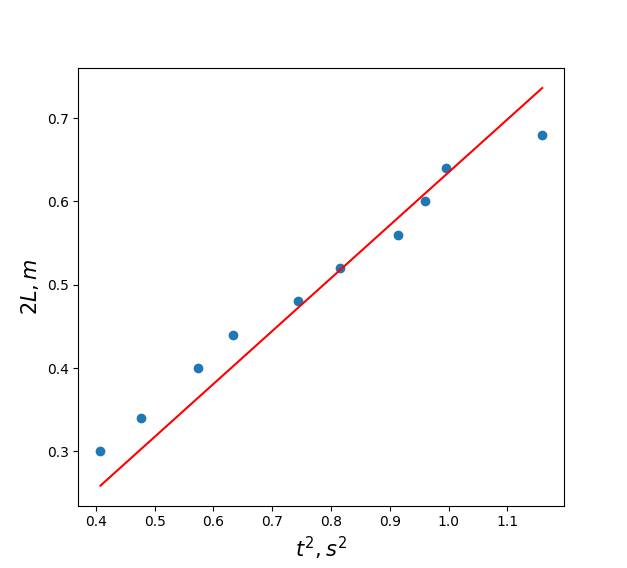
\includegraphics[width=\columnwidth, keepaspectratio=true]{Figure_1.png}
\end{figure}

\subsection{Измерване на земното ускорение - част 1}
В експеримента ще използваме $h=0.2m, \  L=0.2m$. 
\begin{figure}[H]
    \centering
    \caption{}
    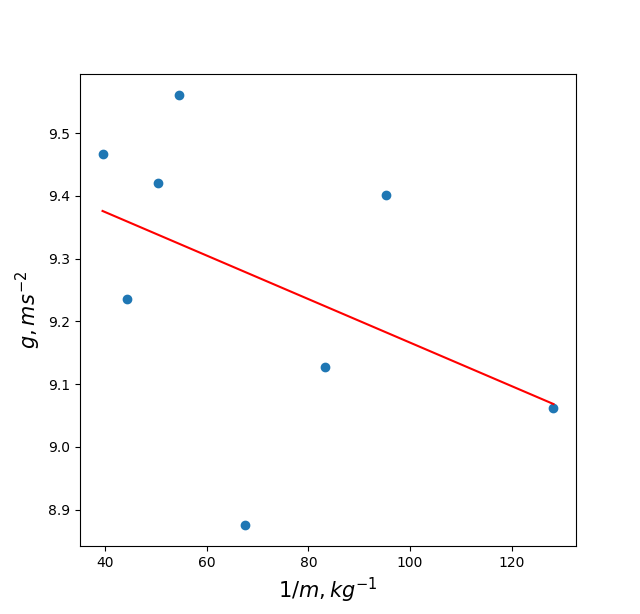
\includegraphics[width=\columnwidth, keepaspectratio=true]{Figure_2.png}
\end{figure}
На Фигура 2 е представена графика на $y=g$ като функция на $x=1/m$. Ако екстраполираме тази зависимост до $x=0 \Rightarrow m=\infty$ получаваме стойност $g=9.51 ms^{-2}$. Тази стойност е най-точна защото при $m \rightarrow \infty$ инерчният момент на макарата не оказва влияние. 

\subsection{Измерване на земното ускорение - част 2}
На Фигура 3 е дадена графиката на $y=\frac{2(2M + M)}{t^2}$ като функция на $x=\frac{m}{L}$. Ъгловият й коефициент е $\frac{dy}{dx}=14.2 ms^{-2}$. Тази стойност не е близо до истинската стойност на земното ускорение, което значи, че този метод за определянето му не е надежден. 
\begin{figure}[H]
    \centering
    \caption{}
    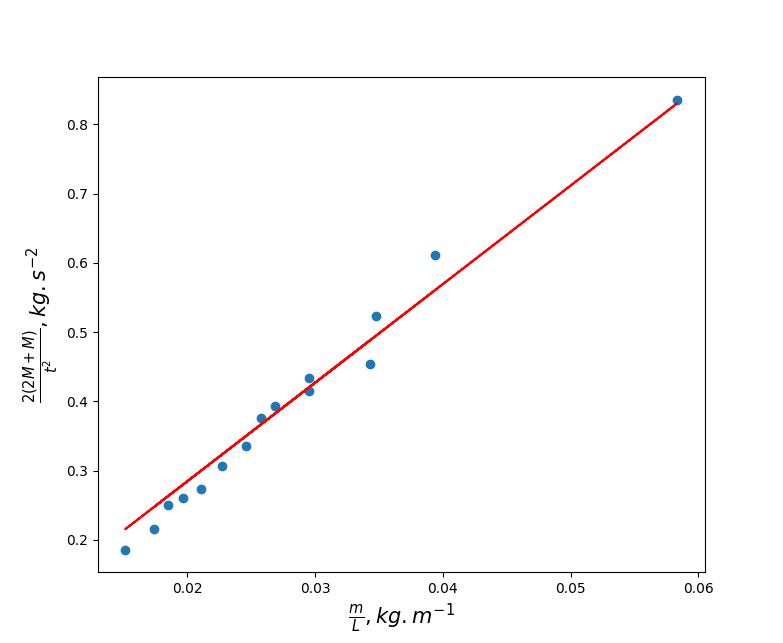
\includegraphics[width=\columnwidth, keepaspectratio=true]{Figure_3.png}
\end{figure}

\end{document}